\documentclass{article}
\usepackage{graphicx,hyperref, calc}
\usepackage[super]{nth}

\setlength{\textwidth}{6.5in}
\setlength{\textheight}{8.25in}
\setlength{\oddsidemargin}{0in}
\setlength{\evensidemargin}{0in}
\setlength{\parskip}{2ex}
\setlength{\parindent}{0in}

\newcommand{\Rin}[1]{\textbf{$>$ {#1}}}
\newcommand{\Rcom}[1]{\hspace{1cm} \#{#1}}
\newcommand{\Rout}[1]{\texttt{{#1}}}

\begin{document}
\pagestyle{myheadings}\markright{
CU Boulder \hspace{0.5in} MATH 2510 - Introduction to Statistics}


\newpage
%Tutorial 
\begin{center}
\textbf{\underbar{R Tutorial}}
\end{center}

This tutorial will give you a \underbar{brief} introduction to the R-environment using RStudio.  You will be provided with precise R-commands to enter and the corresponding output it should yield (if any).  

The command prompt for the R-environment is a ``greater than" symbol ($>$).  Following a command, comments are often included to indicate the function of the code.  Comments are set off by a pound symbol (\#).  In the exercises that follow, R-code will be written in boldface type with the prompt included as follows:
\begin{center}
\Rin{This is an example of R-code typeset} \Rcom{and this is the corresponding comment}
\end{center}
When appropriate, the resulting output that should appear in R will also be included in the exercise with the following typeset:
\begin{center}
\Rout{[1] This is what the output will look like}.
\end{center}

\begin{enumerate}
\item To assign a name to an object, you can use an equal sign ($=$), a left-arrow ($<$-), or a right-arrow (-$>$).
	\begin{enumerate}
	\item \Rin{a = 15} \Rcom{This assigns to the object `a' the value 15} 
	
	\Rin{a} \Rcom{To look at the object, enter the name} 
	
	\Rout{[1] 15} 
	
	\item \Rin{b $<$- 3+7} \Rcom{Here we include simple arithmetic in the assignment} 
	
	\Rin{b} 
	
	\Rout{[1] 10}
	
	\item \Rin{``Colorado" -$>$ c} \Rcom{Of course, not all data is numerical} 
	
	\Rin{c} 
	
	\Rout{[1] ``Colorado''}
	\end{enumerate}
	
\item To create a list (or array) of data values, you can use the \texttt{c} command.  Basic functions can then be applied to the array.

	\begin{enumerate}
	\item \Rin{x = c(1, 3, 3, 7)} \Rcom{The object x is a list of 4 data values} 
	
	\Rin{x} 
	
	\Rout{[1] 1 3 3 7}
	
	\item \Rin{x = c(x, 2, 5)} \Rcom{And two more data values have been added to x} 
	
	\Rin{x} 
	
	\Rout{[1] 1 3 3 7 2 5}
	\item \Rin{length(x)} \Rcom{This command computes the number of elements in x.} 
	
	\Rout{[1] 6}
	
	\item \Rin{x[5]} \Rcom{We can look at just the 5th element in the list.} 
	
	\Rout{[1] 2}
	
	\item \Rin{mean(x)} \Rcom{Some statistics can be computed.} 
	
	\Rout{[1] 3.5}
	
	\item \Rin{xave = mean(x)} \Rcom{The value of the mean of the list x is assigned the name `xave'} 
	
	\Rin{xave} \Rcom{Now we must call the object name to see the output value.} 
	
	\Rout{[1] 3.5}
	\end{enumerate}
	
\item To save our progress (to return later or to submit for grading), all the objects in the workspace need to be saved as is.  It is strongly recommended that you attempt to save this tutorial workspace now, quit R, reopen R, and reload the saved workspace.
	\begin{itemize}

	\item R-Studio: In R-Studio, there is a ``Session" menu which includes a ``Save Workspace As..." option.  Use this to save your workspace now.  Once saved, quit R-Studio and restart the application.
	
    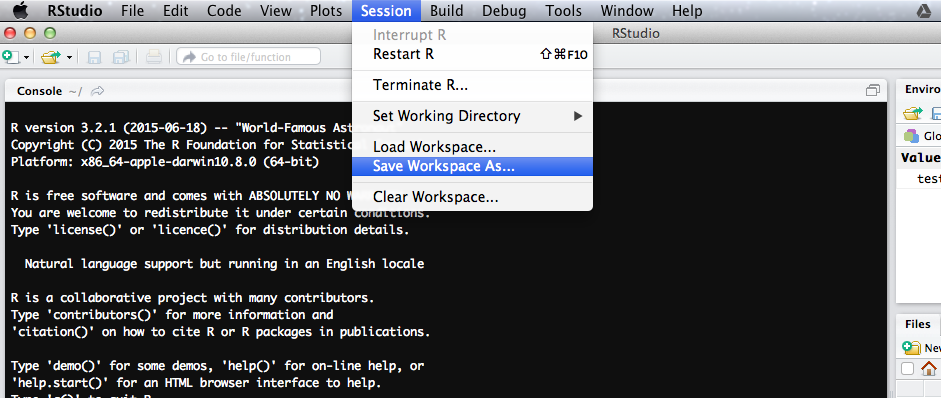
\includegraphics[width=\textwidth-1.65cm]{RSave.png}
	
	\item Now load that saved workspace by using the ``Load Workspace..." option under the ``Session" menu.
	
	 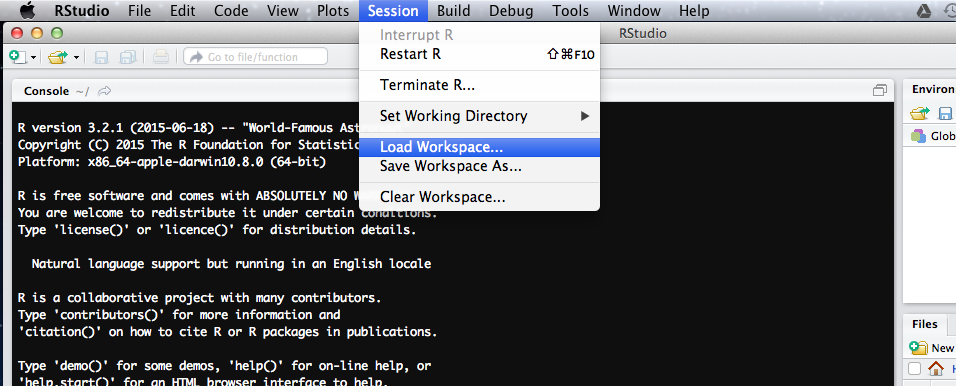
\includegraphics[width=\textwidth-1.65cm]{RLoad.png}
	 
	\end{itemize}
	Check that you have reloaded the saved data correctly. \\
	\Rin{length(x)}\\
	\Rout{[1] 6}\\
	\Rin{b}\\
	\Rout{[1] 10}

\newpage

\item When in the R-environment, the up- and down-arrow keys can be used to scroll through previously entered lines of code.  This can be especially useful if you want to re-execute a command or realize that there is a typo and can then just fix the typo rather than retype the enter line of code.
	\begin{enumerate}
	\item The following code searches a list Y for the first occurrence of the data value $7$ and returns the location of that first $7$. 
	
	\Rin{Y = c(5, 2, 4, 4, 5, 8, 2, 4, 6, 7, 2, 1, 7, 2, 9, 4)} \Rcom{We can see the first $7$ is the \nth{10} element.} 
	
	\Rin{n = 1} \Rcom{We will start the search with element number 1 in the list} 
	
	\Rin{while(Y[n] != 7)\{n=n+1\}} \Rcom{We check each element of Y until the value equals 7.} 
	
	\Rin{n} \Rcom{We call for the value of n.} 
	
	\Rout{[1] 10} 
	
	\item At this point having just run the code to find the first occurrence of the value $7$, you realize that you really want the first occurrence of the value $8$.  Rather than retype all 5 lines, use the arrow keys to recall (and edit, as necessary). 
	
	Arrow up 3 times to \Rin{n=1} \Rcom{Restart the search from the start of the list.} 
	
	Arrow up 3 times to \Rin{while(Y[n] != 7)\{n=n+1\}} 
	\Rcom{But use the back-arrow to get to the 7, backspace and type 8, then enter.} 
	
	Arrow up 3 times to \Rin{n} 
	
	\Rout{[1] 6}
	\end{enumerate}
\end{enumerate}

\end{document}
